
\hspace{20 px} Since Bernhard Riemann, mathematicians knew that a geometric hyperbolic surface can be described with only a finite number of parameters. Knowing this, for a given surface, we can be interested in the set of all geometries we can give it, modulo composition by map isotopic to the identity map, this set is called the Teichmuller space. Other problems rise shortly after this definition. How can we deform in a natural way a surface's geometry into another? What does it mean that a geometry is close to another? What are the natural boundaries of the Teichmuller space?

\begin{wrapfigure}{r}{5cm}
  \centering
  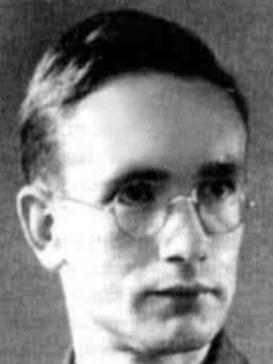
\includegraphics[width=4cm]{Image/Teichmuller.jpeg}
  \caption{The mathematician Oswald Teichmuller}
\end{wrapfigure}

\vspace{10 px}

Oswald Teichmuller, a german mathematician, studied and answered this question in the year preceding the second World War. He created the first metric on this space by finding a solution to an extremal problem: between two hyperbolic geometry on the same surface is there a function which minimize the deformation ? The resulting theorem \cite{teichmuller1940extremale} proves not only the existence, but also the unicity of this function. It naturally induced a distance in the now called Teichmuller space by considering the logarithm of the deformation of the extremal function.

\vspace{10 px}

Thurston then added other important steps to this theory. He underlined the role of laminations. A lamination is a generalisation of simple closed curve. And he introduced the earthquake flow, in a course in 1976-1977 at Priceton, which plays an important role in Teichmuller theory .
Kerckhoff used this tool to show the Nielsen realisation conjecture in 1983 \cite{NielsenRealizationPro} which states that every finite subgroup of the mapping class group have a fixed point in the Teichmuller space.
This theory have been actively studied and therefore generated a lot of literature and contributions. One can refer to the following books \cite{farb2011primer}, \cite{hubbardhal01297628}, \cite{kapovich2009hyperbolic} or course notes \cite{Mcmullen1998HyperbolicM} \cite{Mcmullen1998Riemann} for a more detailed study of the theory.

\vspace{10 px}

Still, some questions remain open, raising further interest of the community in the topic of hyperbolic geometry.
Among the main questions encountered, figures the asymptotic number of closed geodesics. To begin with, one can wonder what is the number $\pi(X,L)$ of closed geodesic on a hyperbolic surface $X$ of length less than $L$. The answer was found in the 1940s and 1950s by Delsarte, Huber and Selberg and -due to its resemblance to the prime number theorem- is called the prime number theorem for hyperbolic surfaces. It states that:\[
\pi(X,L) \simeq e^{L} / L
\]
as $L \to \infty$. The reader can refer to \cite{buser2010geometry} for more details.\\

A much harder problem was to find the number, $\sigma(X,L)$, of simple (which don't intersect themselves) closed geodesic of length less than $L$ on a hyperbolic surface $X$. It was found years later, in Mirzakhani's PhD \cite{mirzakhani2004simple}, and we have \[
\sigma(X,L) \simeq C_{X}L^{6g-6}
\]
As $L \to \infty$ where $g$ is the genus of the surface $X$ and $C_{X}$ is a constant which depend of the geometry $X$.\\
To obtain such a result, Maryam Mirzakhani conjugated the earthquake flow to the horocycle flow. This step provides that the Earthquake flow is ergodic and allows us to use Birkoff theorem to understand asymptotic quantities.

\vspace{10 px}

The question is now to give error terms to this quantity. In order to do that, we need to understand better the mixing rate of the earthquake flow. This flow is conjugate to the horocyclic flow which has a polynomial mixing rate. But as the conjugacy is only a measurable map it transport the rate of mixing on a subset of the $L^2$ of the moduli space which could be diffult to use. We should analyse the rate of mixing of the earthquake flow by other means. One research direction would be to consider natural functions on Teichmuller space such as the systole. The systole is the lenth of the shortest simple closed curve on the surface. This function behaves nicely along earthquake path, it is continuous, convex and we know its first derivative at the origin. Moreover in the case of the once punctured torus we can give a frame determined by the continued fraction of the slope.

\vspace{10 px}

In this master thesis, I will first give an introduction to Teichmuller theory and some useful and classical tools in this theory such as the collar lemma or a surface's decomposition in pair of pants. Then, we will review the proof of the Mirzakhani's conjugacy between the horocyclic flow and the earthquake flow. After doing so, we will focus on the mixing properties of the geodesic and horocyclic flow, and discuss their mixing rate. Finally we will discuss a special case: the once punctured torus, as it is one of the simplest example of hyperbolic surface.
